\documentclass[a4paper, 14pt]{article}
\usepackage[utf8]{inputenc}
\usepackage[russian]{babel}
\usepackage{graphicx}
\usepackage{listings}
\usepackage{color}
\usepackage{amsmath}
\usepackage{pgfplots}
\usepackage{url}
% подключаем hyperref (для ссылок внутри  pdf)
\usepackage[unicode, pdftex]{hyperref}
\usepackage[T2A]{fontenc}
\usepackage[utf8]{inputenc}
\lstset{tabsize=2,
    breaklines,
    columns=fullflexible,
    flexiblecolumns,
    numbers=left,
    keepspaces=true,
    numberstyle={\footnotesize},
    extendedchars=\true
}
\lstdefinelanguage{MyC}{
  language=C++,
  ndkeywordstyle=\color{darkgray}\bfseries,
  identifierstyle=\color{black},
  morecomment=[n]{/**}{*/},
  commentstyle=\color{blue}\ttfamily,
  stringstyle=\color{red}\ttfamily,
  morestring=[b]",
  showstringspaces=false,
  morecomment=[l][\color{gray}]{//},
  keepspaces=true,
  escapechar=\%,
  %texcl=⟨true|false⟩
}
%\usepackage[russian,russian,english]{babel}
\frenchspacing                    % ставим пробелы в соответствии с французским стилем
\DeclareGraphicsExtensions{.pdf,.png,.jpg,.svg}
\usepackage{titlesec}
\usepackage{algpseudocode}
\usepackage{caption}
\usepackage{setspace}
\usepackage[linesnumbered,boxed]{algorithm2e}



\DeclareCaptionFont{white}{\color{white}} %% это сделает текст заголовка белым
%% код ниже нарисует серую рамочку вокруг заголовка кода.

\linespread{1}

\DeclareCaptionFormat{listing}{\colorbox{gray}{\parbox{\textwidth}{#1#2#3}}}
\captionsetup[lstlisting]{format=listing,labelfont=white,textfont=white} 

\begin{document}
	\begin{titlepage}
		\begin{center}
			\begin{LARGE}
				Отчет по лабораторной работе №6\\
					по курсу "Анализ алгоритмов"\\
					по теме "Муравьиные алгоритмы"
			\end{LARGE}
		
			\begin{Large}
				\vspace{10cm}
				Студент: Доктор А.А. ИУ7-53\\
					Преподаватель: Волкова Л.Л.,
								   Строганов Ю.В.\\
				
				\vspace{5cm}2018 г.				   
			\end{Large}
			
		\end{center}
		 
	\end{titlepage}

\tableofcontents
	
\newpage
\section*{Введение}
\addcontentsline{toc}{section}{Введение}
\hspace{1cm}

Муравьиный алгоритм (алгоритм оптимизации подражанием муравьиной колонии, англ. ant colony optimization, ACO) — один из эффективных полиномиальных алгоритмов для нахождения приближённых решений задачи коммивояжёра, а также решения аналогичных задач поиска маршрутов на графах. Суть подхода заключается в анализе и использовании модели поведения муравьёв, ищущих пути от колонии к источнику питания и представляет собой метаэвристическую оптимизацию. Первая версия алгоритма, предложенная доктором наук Марко Дориго в 1992 году, была направлена на поиск оптимального пути в графе\cite{ant_description}.

В реальном мире муравьи (первоначально) ходят в случайном порядке и по нахождении продовольствия возвращаются в свою колонию, прокладывая феромонами тропы. Если другие муравьи находят такие тропы, они, вероятнее всего, пойдут по ним. Вместо того, чтобы отслеживать цепочку, они укрепляют её при возвращении, если в конечном итоге находят источник питания. Со временем феромонная тропа начинает испаряться, тем самым уменьшая свою привлекательную силу. Чем больше времени требуется для прохождения пути до цели и обратно, тем сильнее испарится феромонная тропа. На коротком пути, для сравнения, прохождение будет более быстрым и как следствие, плотность феромонов остаётся высокой. Испарение феромонов также имеет свойство избежания стремления к локально-оптимальному решению. Если бы феромоны не испарялись, то путь, выбранный первым, был бы самым привлекательным. В этом случае, исследования пространственных решений были бы ограниченными. Таким образом, когда один муравей находит (например, короткий) путь от колонии до источника пищи, другие муравьи, скорее всего пойдут по этому пути, и положительные отзывы в конечном итоге приводят всех муравьёв к одному, кратчайшему, пути\cite{ant_info}. На рис.  \ref{ris:ant_run} продемонстрирован принцип устройства муравьиного подхода\cite{ant_work_image}.


\begin{figure}[h]
\center
\includegraphics[scale=0.3]{ant_run.png}
\caption{Принцип работы муравьиного алгоритма}
\label{ris:ant_run}
\end{figure}

\newpage
Задача коммивояжёра (англ. Travelling salesman problem, сокращённо TSP) — одна из самых известных задач комбинаторной оптимизации, заключающаяся в поиске самого выгодного маршрута, проходящего через указанные города хотя бы по одному разу с последующим возвратом в исходный город. В условиях задачи указываются критерий выгодности маршрута (кратчайший, самый дешёвый, совокупный критерий и тому подобное) и соответствующие матрицы расстояний, стоимости и тому подобного. Как правило, указывается, что маршрут должен проходить через каждый город только один раз — в таком случае выбор осуществляется среди гамильтоновых циклов. Существует несколько частных случаев общей постановки задачи, в частности, геометрическая задача коммивояжёра (также называемая планарной или евклидовой, когда матрица расстояний отражает расстояния между точками на плоскости), метрическая задача коммивояжёра (когда на матрице стоимостей выполняется неравенство треугольника), симметричная и асимметричная задачи коммивояжёра. Также существует обобщение задачи, так называемая обобщённая задача коммивояжёра.

Оптимизационная постановка задачи относится к классу NP-трудных задач, впрочем, как и большинство её частных случаев. Версия «decision problem» (то есть такая, в которой ставится вопрос, существует ли маршрут не длиннее, чем заданное значение k) относится к классу NP-полных задач. Задача коммивояжёра относится к числу трансвычислительных: уже при относительно небольшом числе городов (66 и более) она не может быть решена методом перебора вариантов никакими теоретически мыслимыми компьютерами за время, меньшее нескольких миллиардов лет.

На рис. \ref{ris:kommi} представлен оптимальный маршрут коммивояжёра через 15 крупнейших городов Германии. Указанный маршрут является самым коротким из всех возможных 43 589 145 600 вариантов.

\begin{figure}[h]
\center
\includegraphics[scale=0.8]{kommi.png}
\caption{оптимальный маршрут коммивояжёра через 15 крупнейших городов Германии}
\label{ris:kommi}
\end{figure}


\newpage
\section*{Задачи работы}

В ходе выполнения данной лабораторной работы, мной были выполнены следующие задачи:

\begin{enumerate}
\item[1)] С помощью одного из муравьиных алгоритмов решить задачу коммивояжёра;
\item[2)] провести замеры скорости работы работы алгоритма при разных коэффициентах(влияния расстояний\феромонов), количестве поколений и элитных муравьев.
\end{enumerate}


\newpage
\section{Аналитическая часть}
\hspace{1cm}	В данном разделе приведено описание оригинального муравьиного алгоритма и несколько способов его улучшения

\subsection {Оригинальный муравьиеый алгоритм} \\

Каждый муравей хранит в памяти список пройденных им узлов. Этот список называют списком запретов (tabu list) или просто памятью муравья. Выбирая узел для следующего шага, муравей «помнит» об уже пройденных узлах и не рассматривает их в качестве возможных для перехода. На каждом шаге список запретов пополняется новым узлом, а перед новой итерацией алгоритма – то есть перед тем, как муравей вновь проходит путь – он опустошается.

Кроме списка запретов, при выборе узла для перехода муравей руководствуется «привлекательностью» ребер, которые он может пройти. Она зависит, во-первых, от расстояния между узлами (то есть от веса ребра), а во-вторых, от следов феромонов, оставленных на ребре прошедшими по нему ранее муравьями. Естественно, что в отличие от весов ребер, которые являются константными, следы феромонов обновляются на каждой итерации алгоритма: как и в природе, со временем следы испаряются, а проходящие муравьи, напротив, усиливают их\cite{ant_habr}.

Пусть муравей находится в узле , а узел  – это один из узлов, доступных для перехода: . Обозначим вес ребра, соединяющего узлы  и , как , а интенсивность феромона на нем – как . Тогда вероятность перехода муравья из  в  будет равна:

\begin{equation}\label{form:way} 
 p_{i,j}={\frac {(\tau _{i,j}^{\alpha })(\eta _{i,j}^{\beta })}{\sum (\tau _{i,j}^{\alpha })(\eta _{i,j}^{\beta })}}
 \end{equation}
 \begin{align*}
    \text{где} \\
   \tau _{i,j} &- \text{ расстояние от города i до j;} \\
    \eta _{i,j} &- \text{ количество феромонов на ребре ij;} \\
    \alpha &- \text{параметр влияния длины пути;} \\
    \beta &- \text{параметр влияния феромона.}
\end{align*}

Очевидно, что при {\beta = 0$} алгоритм превращается в классический жадный алгоритм, а при {\alpha = 0$} он быстро сойдется к некоторому субоптимальному решению. Выбор правильного соотношения параметров является предметом исследований, и в общем случае производится на основании опыта.

\vspace{\baselineskip}
После того, как муравей успешно проходит маршрут, он оставляет на всех пройденных ребрах след, обратно пропорциональный длине пройденного пути:
\begin{equation}\label{form:eva} 
    \tau _{i,j}=(1-\rho )\tau _{i,j}+\Delta \tau _{i,j},
\end{equation}
\begin{align*}
    \text{где} \\
    \rho _{i,j} &- \text{доля феромона, который испарится;} \\
    \tau _{i,j} &- \text{количество феромона на дуге ij;} \\
    \Delta \tau _{i,j} &- \text{количество отложенного феромона.}
\end{align*}

Количество отложенного феромона, обычно определяется как:

\begin{equation}\label{form:add} 
    {\displaystyle \Delta \tau _{i,j}^k={\begin{cases}Q/L_{k}& {\mbox{Если k-ый мурваей прошел по ребру ij;}}\\0&{\mbox{Иначе}}\end{cases}}}
\end{equation}
\begin{align*}
    \text{где} \\
    Q &- \text{количество феромона, переносимого муравьем;} \\
    L_{k} &- \text{стоимость k-го пути муравья (обычно длина).}
\end{align*}

\vspace{\baselineskip}

Трудоёмкость муравьиного алгоритма:
\begin{equation}\label{form:complex} 
O(t*m*n^2)
\end{equation}
\begin{align*}
    \text{где} \\
     t &- \text{количество поколений;} \\
     m &- \text{количество муравьев;} \\
     n &- \text{количество городов.} \\
\end{align*}

Ниже приведены вариации муравьиного алгоритма.

\begin{enumerate}

\item \textbf{Элитарная муравьиная система}.
Из общего числа муравьёв выделяются так называемые «элитные муравьи». По результатам каждой итерации алгоритма производится усиление лучших маршрутов путём прохода по данным маршрутам элитных муравьёв и, таким образом, увеличение количества феромона на данных маршрутах. В такой системе количество элитных муравьёв является дополнительным параметром, требующим определения. Так, для слишком большого числа элитных муравьёв алгоритм может «застрять» на локальных экстремумах.

\item \textbf{Max-Min муравьиная система}.
Добавляются граничные условия на количество феромонов (τmax,τmin). Феромоны откладываются только на глобально лучших или лучших в итерации путях. Все рёбра инициализируются значением τmax.

\item \textbf{Ранговая муравьиная система(ASrank)}.
Все решения ранжируются по степени их пригодности. Количество откладываемых феромонов для каждого решения взвешено так, что более подходящие решения получают больше феромонов, чем менее подходящие.

\item \textbf{Длительная ортогональная колония муравьёв (COAC)}.
Механизм отложения феромонов COAC позволяет муравьям искать решения совместно и эффективно. Используя ортогональный метод, муравьи в выполнимой области могут исследовать их выбранные области быстро и эффективно, с расширенной способностью глобального поиска и точностью.

\end{enumerate}
	
		\newpage
	\section{Конструкторская часть}
	\hspace{1cm}В данном разделе будут описаны принципы работы выбранных решений и их блоксхемы.
	\subsection{Разработка реализаций алгоритмов}
	
\hspace{1cm} Основное действие происходит в функции run (рис. \ref{ris:run_1}, \ref{ris:run_2}, \ref{ris:run_3}). На вход ей поступают следующие параметры:
	\begin{enumerate}
	\item[1)] time - количество поколений муравьев;
    \item[2)] \text{ants amount} - количество муравьев;
    \item[3)] elite\_one - каждый i-ый(i = elite one) муравей будет элитным;
    \item[4)] cities - количество городов;
    \item[5)] eva(evaporation) - процент распыления феромона;
    \item[6)] al(alpha) - параметр влияния расстояния;
    \item[7)] be(beta) - параметр влияния феромона;
    \item[8)] city\_from - город появления муравьев;
    \item[9)] Q, EQ - величина феромона обычного и элитного муравьев.
    \end{enumerate}
Они проверяются на корректность в функции run\_check(рис. \ref{ris:run_check}). Затем создаются и инициализируются матрицы дистанций, феромонов, массивы муравьев и начинается главный цикл функции - по поколениям. На этом этапе массив муравьев обновляет значения своих элементов до исходных значений(очищаются списки пройденных городов и пройденное расстояние). Затем начинаем обход муравьев. Сначала добавим родной город в список уже посещенных муравьем, чтобы он не мог 'случайно' заскочить домой, не обойдя все остальные города. Дальше начинается третий(по вложенности) цикл. Пока муравей не обошёл все города(can\_move() - рис. \ref{ris:can_move}), пусть двигается(make\_move - \ref{ris:map_make_move}). После того, как муравей пройдет все города(выход из цикла), вручную добавляем ему расстояние от текущего города(последнего, в котором он оказался) до родного(города рождения) - иначе получается, что домой он так и не попал, что весьма грустно. Также добавляем его родной город в список посещенных(во второй раз!). Это делается для того, чтобы если мы захотим распечатать путь движения муравья, было видно, что он из дома вышел и домой же вернулся. Дальше 'распыляем' феромоны с помощью функции increase\_pheromone - рис. \ref{ris:increase_pheromone}. После чего сравниваем лучшее расстояние, что у нас было(хранится в переменной best\_way) с пройденным расстоянием муравья и с 0(По умолчанию best\_way равен -1). Если одно из этих условий выполняется, обновляем best\_way и tabu\_list(копию муравьиного массива пройденных городов). Иначе просто идём дальше. И последнее наше действие - уменьшение феромонов на карте. Условно считаем, что каждый следующий муравей начинает движение, когда вернулся прошлый, то есть одновременно на карте присутствует только 1 муравей. Тогда не выходя из цикла по муравьям, сразу после проверки на кратчайший путь уменьшим феромоны по всей карте с помощью функции  reduce\_pheromone() - рис. \ref{ris:reduce_pheromone}.
\newpage

\begin{figure}[h!]
\center
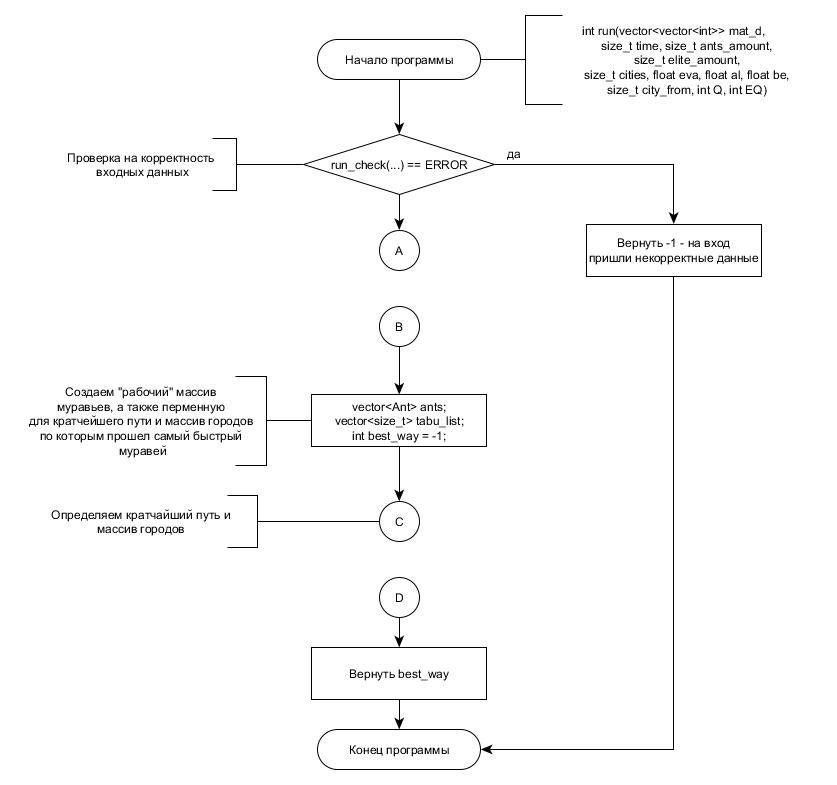
\includegraphics[scale=0.5]{run_1_main.jpg}
\caption{Основная часть функции run.}
\label{ris:run_1}
\end{figure}\newpage

\begin{figure}[h!]
\center
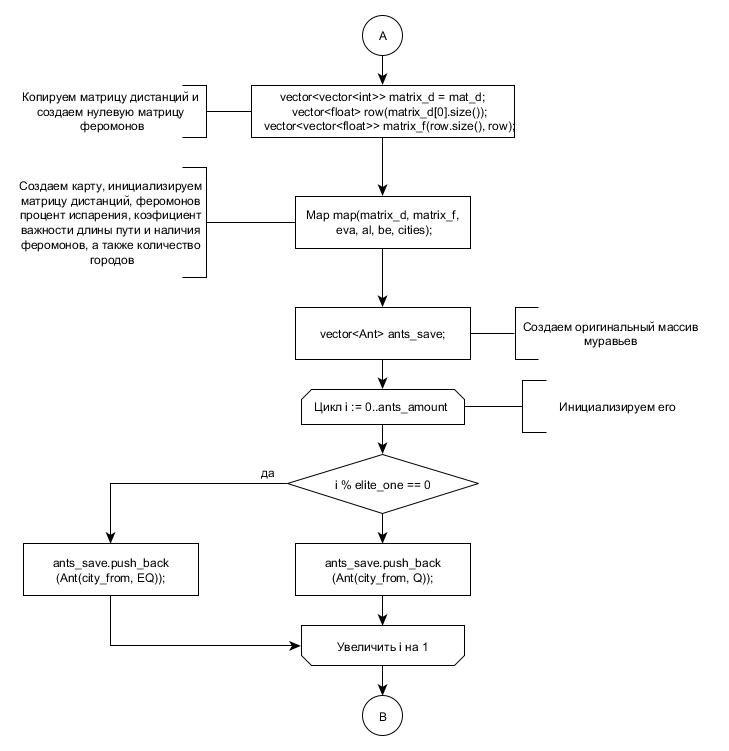
\includegraphics[scale=0.6]{run_2_ab.jpg}
\caption{Инициализация муравьев и матриц.}
\label{ris:run_2}
\end{figure}\newpage

\begin{figure}[h!]
\center
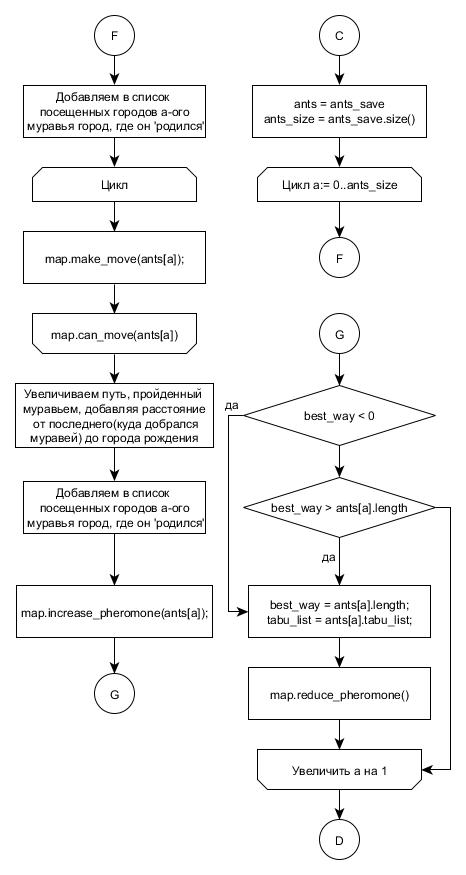
\includegraphics[scale=0.6]{run_3_cd.jpg}
\caption{Процесс поиска кратчайшего пути.}
\label{ris:run_3}
\end{figure}\newpage

\begin{figure}[h!]
\center
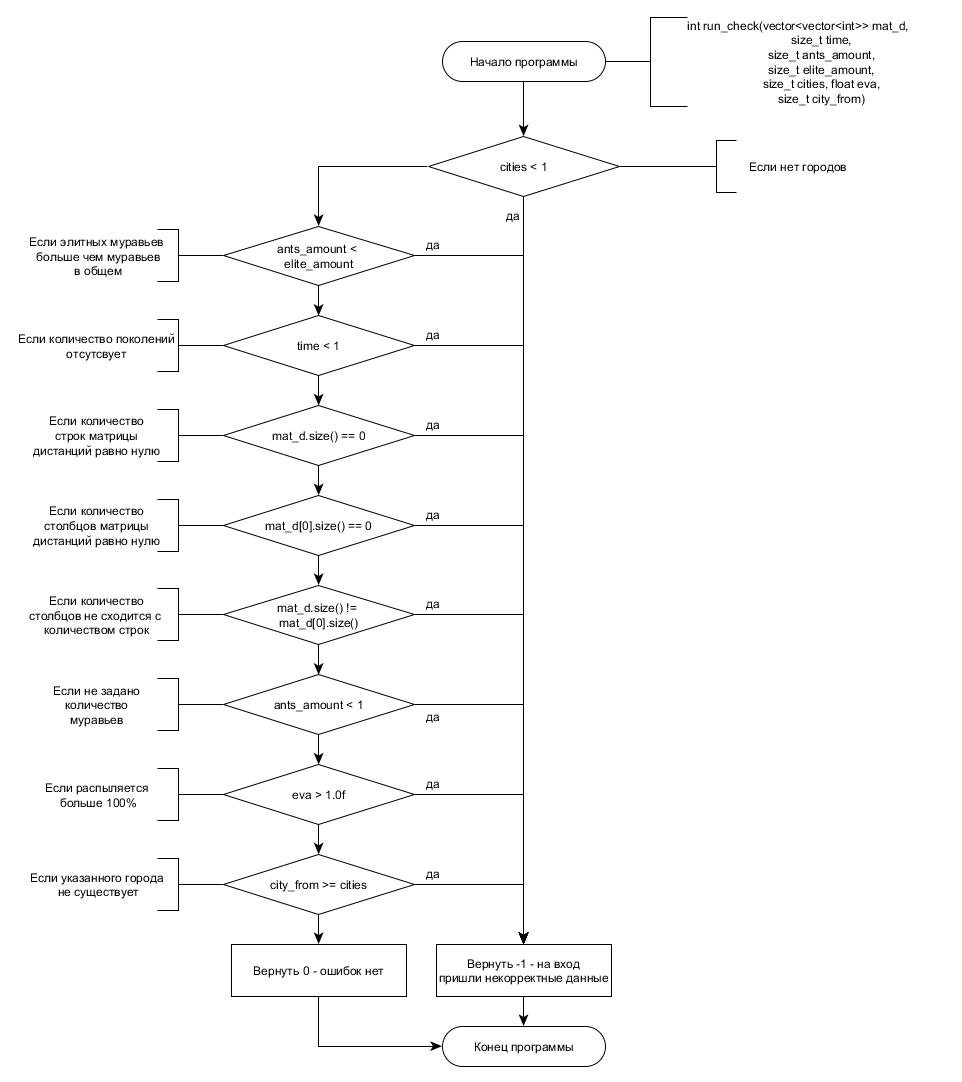
\includegraphics[scale=0.5]{run_check.jpg}
\caption{Проверка корректности входных данных.}
\label{ris:run_check}
\end{figure}\newpage

Функция can\_move(рис. \ref{ris:can_move}) принимает на вход муравья(объект класса Ant - с этого места и дальше просто муравей) и возвращает false(и следовательно прекращает поход муравья), когда размер массива посещенных городов данного муравья становится больше или равен количеству существующих городов. Иначе вернет true и муравей продолжит двигаться. 

\begin{figure}[h!]
\center
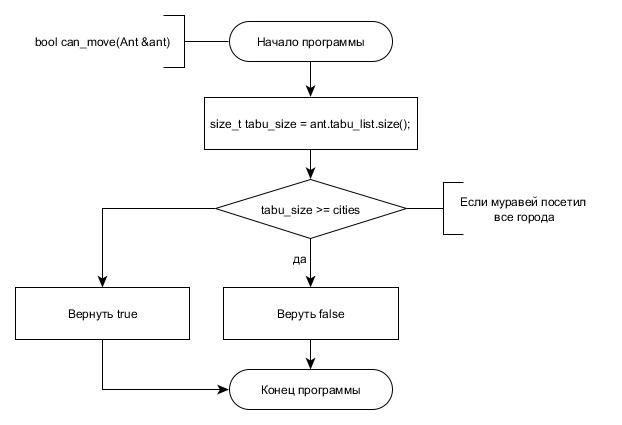
\includegraphics[scale=0.6]{can_move.jpg}
\caption{Функция can\_move.}
\label{ris:can_move}
\end{figure}\newpage

Функция make\_move(рис. \ref{ris:map_make_move}) класса Map принимает на вход муравья и ничего не возвращает. Вначале выполняется поиск(choose\_city() - рис. \ref{ris:choose_city}) следующего города, куда отправится муравью. После чего определяется расстояние до выбранного города(по матрице дистанций) и дальше функция отдает управление самому муравью, а именно его(класса Ant) одноимённой функции make\_move.

\begin{figure}[h!]
\center
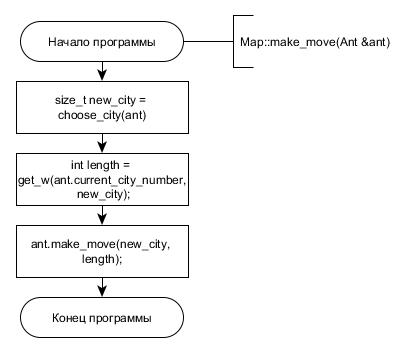
\includegraphics[scale=0.8]{map_make_move.jpg}
\caption{Функция make\_move класса Map.}
\label{ris:map_make_move}
\end{figure}\newpage

Муравьиная функция make\_move(рис. \ref{ris:ant_make_move}) принимает на вход два параметра: следующий город и расстояние до него. Как и своя тёзка - ничего не возвращает. Эта функция последовательно выполняет следующие 3 действия: 

\begin{enumerate}
	\item[1)] помещает номер указанного города в массив посещённых городов;
    \item[2)] обновляет город пребывания муравья;
    \item[3)] увеличивает пройденное расстояние муравья на указанное значение.
\end{enumerate}

\begin{figure}[h!]
\center
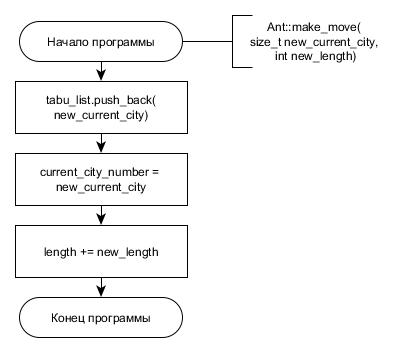
\includegraphics[scale=0.7]{ant_make_move.jpg}
\caption{Функция make\_move класса Ant.}
\label{ris:ant_make_move}
\end{figure}\newpage

Функция choose\_city(рис. \ref{ris:choose_city}), упомянутая в make\_move для Map принимает на вход муравья, а возвращает номер города, который тот 'выбрал' для следующего посещения. Для этого функция получает массив вероятностей(элеемнтом этого массива является пара вида: номер города, вероятность перехода(процент)) выбора каждого из городов. После чего с помощью генератора случайных чисел создаётся число от 0 до 100 и определяется, какому городу принадлежит отрезок, в котором находится данное число. Приведу пример, пусть вероятности попадания в города 1,2,3 равны соответсвенно 30, 60 и 10. Тогда отрезок с 0 по 30 'принадлежит' первому городу, с 31 по 90 - второму, с 90 по 100 - третьму. Например, если число, созданное генератором, равно 95, то муравей пойдкт третий город. Если число равно 40, то пойдет во второй город и т.д. Массив процентов определяется в функции get\_p() - рис. \ref{ris:get_p_1}, \ref{ris:get_p_2}, \ref{ris:get_p_4}, \ref{ris:get_p_3}, о которой пойдет речь дальше.

\begin{figure}[h!]
\center
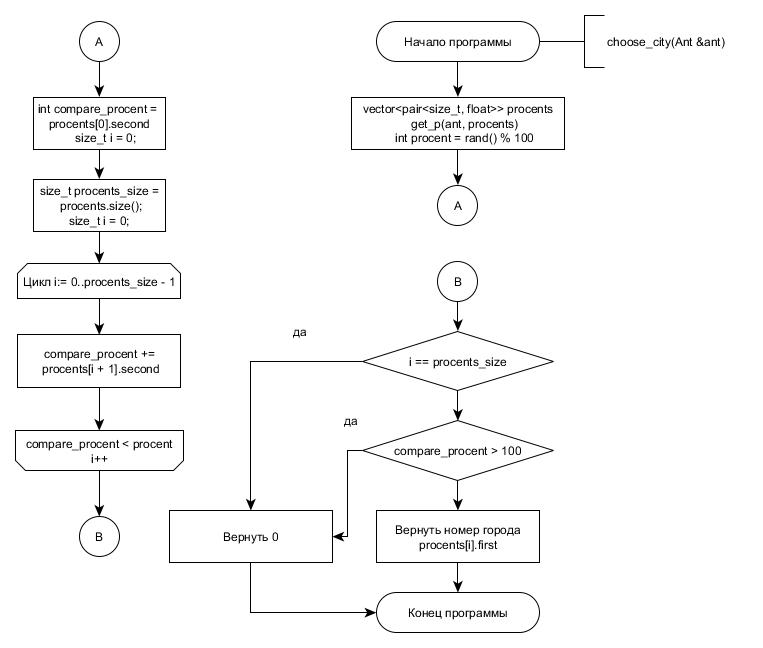
\includegraphics[scale=0.6]{choose_city.jpg}
\caption{Функция choose\_city.}
\label{ris:choose_city}
\end{figure}\newpage

Функция get\_p(рис. \ref{ris:get_p_1}, \ref{ris:get_p_2}, \ref{ris:get_p_3}, \ref{ris:get_p_4}) получает на вход муравья и ссылку на массив вероятностей. Результатом работы будет обновление этого массива. Первым делом массив вероятностей обнуляется. После чего начинается процесс его заполнения. Проходим по всем городам и проверяем, был ли указанный(пришедший на вход) муравей в i-ом городе. Если был, переключаемся на следующий город, если нет, то вычисляем вероятность похода в этот город. Но перед этим уточняем, что i-ый город не является городом пребывания муравья, для этого достаточно проверить, что путь из текущего города в i-ый не равен нулю. Вероятность определяется по формуле \ref{form:way}. Числитель этой формулы вынесен в отдельную функцию get\_p\_chisl(рис. \ref{ris:get_p_chisl}). По определению вероятность - это отношение исходов некоторого события к общему количеству исходов. На данный момент у нас есть только числитель формулы \ref{form:way}, т. е. мы посчитали на самом деле количество исходов события перехода в i-ый город. Не хватает общего количества исходов. Для того, чтобы посчитать это количество, определим за пределами цикла переменную summ и при каждом вычислении кол-ва исходов для определенного города будем прибавлять это значение к summ. При этом будем сохранять кол-во исходов для определенного города в массив вероятностей procents. После того, как мы обойдем все города, на всякий случай, проверим, что наша переменная summ не ноль(чтобы избежать деления на ноль), а дальше пройдемся по массиву procents и поделим каждое значение на summ. Готово, проценты посчитаны, блоксхемы ниже.\newpage

\begin{figure}[h!]
\center
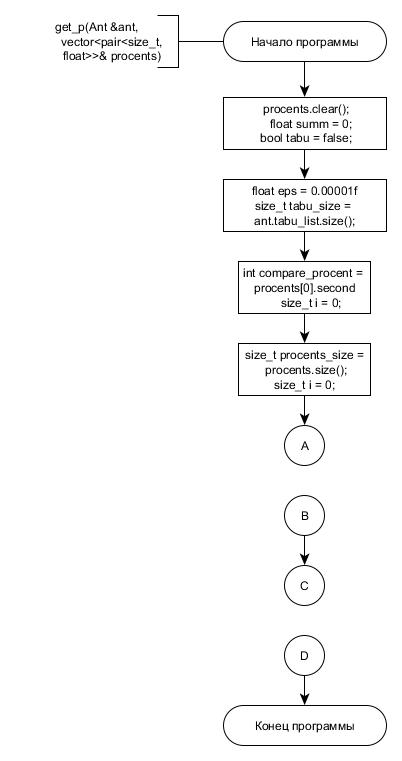
\includegraphics[scale=0.6]{get_p_1_main.jpg}
\caption{Основная часть функции get\_p.}
\label{ris:get_p_1}
\end{figure}\newpage

\begin{figure}[h!]
\center
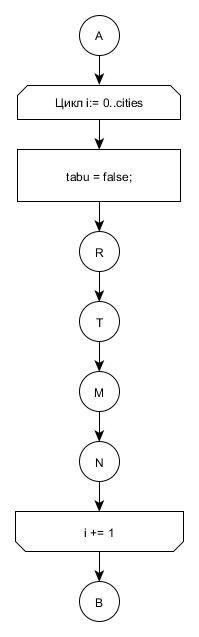
\includegraphics[scale=0.7]{get_p_2_ab.jpg}
\caption{Цикл по всем городам}
\label{ris:get_p_2}
\end{figure}\newpage

\begin{figure}[h!]
\center
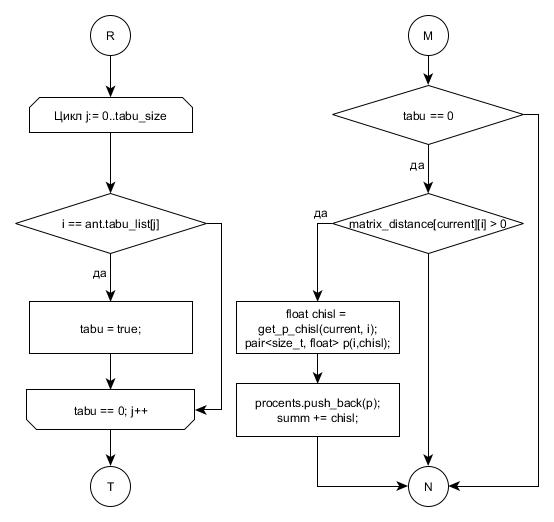
\includegraphics[scale=0.6]{get_p_4_rtmn.jpg}
\caption{Определение является ли город посещенным и занесение в массив процентов числителей вероятностей.}
\label{ris:get_p_4}
\end{figure}\newpage

\begin{figure}[h!]
\center
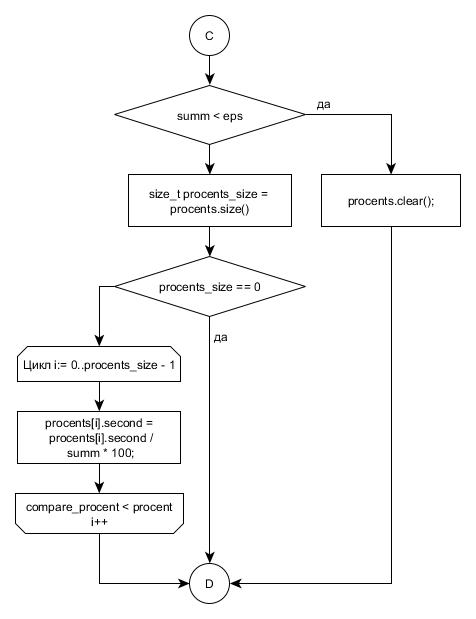
\includegraphics[scale=0.6]{get_p_3_cd.jpg}
\caption{Деление числа исходов событий на общее количество.}
\label{ris:get_p_3}
\end{figure}\newpage

\begin{figure}[h!]
\center
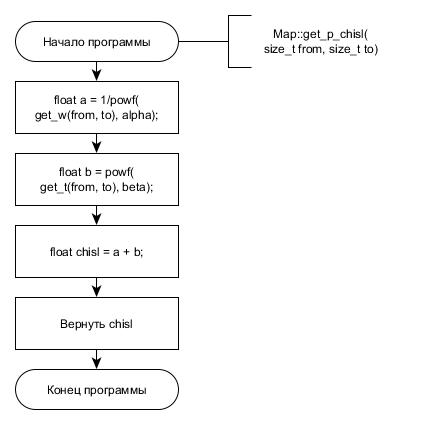
\includegraphics[scale=0.6]{get_p_chisl.jpg}
\caption{Программная реализация числителя формулы \ref{form:way}.}
\label{ris:get_p_chisl}
\end{figure}\newpage

Нерассмотренными остались две функции -  reduce\_pheromone(рис. \ref{ris:reduce_pheromone}) и 
increase\_pheromone(рис. \ref{ris:increase_pheromone}).  Кратко о каждой из них. Первая уменьшает количество феромона. Обходим матрицу феромонов и согласно формуле \ref{form:eva} каждое значение умножаем на процент оставшегося феромона = (1 - коэффициент испарения). Однако по формуле \ref{form:eva} к каждому значению надо еще прибавить некоторое число, но я решил вынести это действие в отдельную функцию, а именно в increase\_pheromone. Эта функция получает на вход муравья и проходит по массиву пройденных им городов. На каждом шаге выделяет 2 города: прошлый(p) и текущий(c). После чего обновляет ячейку [p][c] и [c][p] в матрице феромонов согласно первому случаю из формулы \ref{form:add} - прибавляет к ячейке отношение муравьиного феромена к пройденному расстоянию. Таким образом это компенсирует недостающее слагаемое из формулы \ref{form:eva}.\newpage

\begin{figure}[h!]
\center
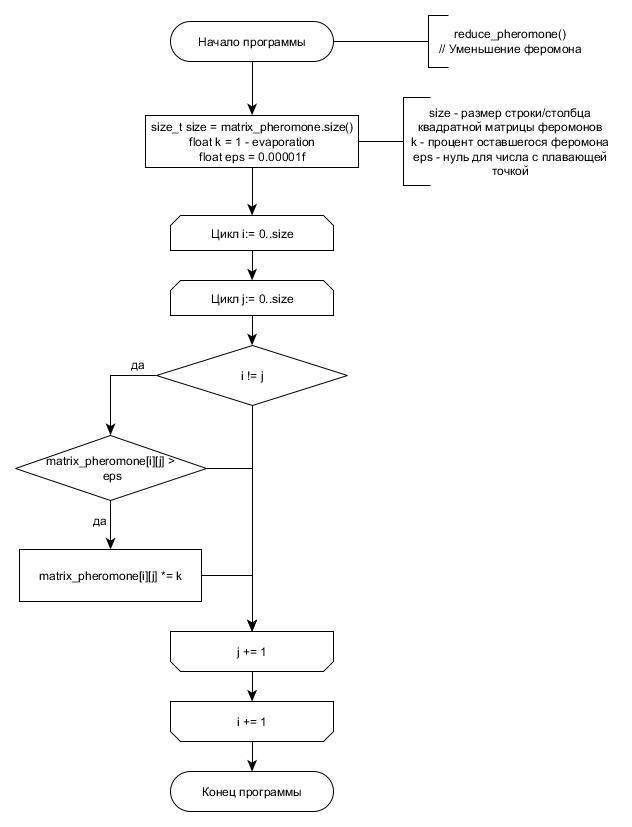
\includegraphics[scale=0.6]{reduce_pheromone.jpg}
\caption{Функция reduce\_pheromone.}
\label{ris:reduce_pheromone}
\end{figure}\newpage

\begin{figure}[h!]
\center
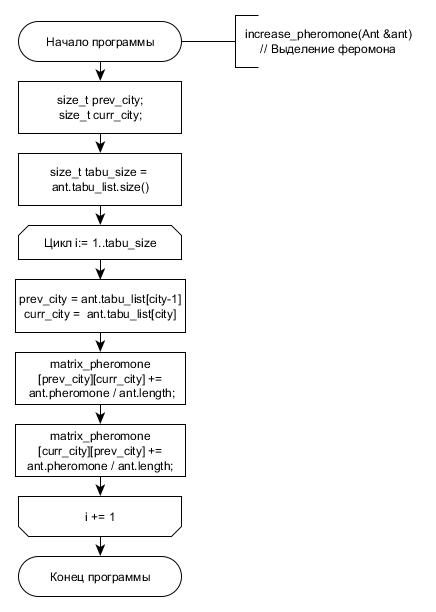
\includegraphics[scale=0.8]{increase_pheromone.jpg}
\caption{Функция increase\_pheromone.}
\label{ris:increase_pheromone}
\end{figure}\newpage

	\newpage
	\section{Технологическая часть}
	\hspace{1cm}В данном разделе будут определены средства реализации и приведен листинг кода.
	

	\subsection{Средства реализации}
	\hspace{1cm}Для реализации программ мною был выбрал язык программирования - C++, поскольку имею опыт работы с ним. 
	Среда разработки - Qt.
	Время работы процессора замерялось с помощью функции, продемонстрированной в листинге \ref{time}. Эта функция в отличие от встроенной функции таймера, способна считать реальное процессорное время работы программы в тиках \cite{lom}. Для ее работы была подключена библиотека time.h.
	\lstset{ %
        language=c++,                 % выбор языка для подсветки (здесь это С)
        basicstyle=\small\sffamily, % размер и начертание шрифта для подсветки кода
        numbers=left,               % где поставить нумерацию строк (слева\справа)
        numberstyle=\tiny,           % размер шрифта для номеров строк
        stepnumber=1,                   % размер шага между двумя номерами строк
        numbersep=-5pt,                % как далеко отстоят номера строк от         подсвечиваемого кода
        backgroundcolor=\color{white}, % цвет фона подсветки - используем         \usepackage{color}
        showspaces=false,            % показывать или нет пробелы специальными     отступами
        showstringspaces=false,      % показывать или нет пробелы в строках
        showtabs=false,             % показывать или нет табуляцию в строках
        frame=single,              % рисовать рамку вокруг кода
        tabsize=2,                 % размер табуляции по умолчанию равен 2 пробелам
        captionpos=t,              % позиция заголовка вверху [t] или внизу [b] 
        breaklines=true,           % автоматически переносить строки (да\нет)
        breakatwhitespace=false, % переносить строки только если есть пробел
        escapeinside={\%*}{*)},   % если нужно добавить комментарии в коде
	    keywordstyle=\color{blue}\ttfamily,
	    stringstyle=\color{red}\ttfamily,
	    commentstyle=\color{green}\ttfamily,
	    morecomment=[l][\color{magenta}]{\#},
	    columns=fullflexible
    }
	\begin{lstlisting}[label=time,caption=Функция замера процессороного времени]
    unsigned long long tick(void)
    {
        unsigned long long d;
        __asm__ __volatile__ ("rdtsc" : "=A"     (d));
        return d;
    }
	\end{lstlisting}

	\newpage
	\subsection{Реализация алгоритмов}
	
	Для реализации описанных в конструкторской части решений, было реализовано два класса: Map(листинг \ref{code:map_class}) и Ant(листинг  \ref{code:ant_class}).
		\begin{lstlisting}[label=code:map_class,caption=Класс Map]
    class Map {
    public:
        Map(vector<vector<int>> matrix_d,
            vector<vector<float>> matrix_p,
            float eva, float al, float be, size_t ci) :
        matrix_distance(matrix_d), matrix_pheromone(matrix_p),
        evaporation(eva), alpha(al), beta(be), cities(ci){;}
    
        // Матрица дистанций и феромонов
        vector<vector<int>> matrix_distance;
        vector<vector<float>> matrix_pheromone;
    
        // Интенсивность испарения. От 0 до 1.
        float evaporation;
        // Важность веса ребра и уровня феромонов соответственно
        float alpha, beta;
        // Количество городов
        size_t cities;
    
        // Возвращает ложь, если пройдены все города, иначе истину
        bool can_move(Ant &ant) {
            size_t tabu_size = ant.tabu_list.size();
            if (tabu_size >= this->cities) {
                return false;
            }
            return true;
        }
    
        // Уменьшение феромона
        void reduce_pheromone();
    
        // Выделение нового феромона
        void increase_pheromone(Ant &ant);
    
        // Обновить данные муравья
        void make_move(Ant &ant);
    
    private:
        // Получить массив исходов
        float get_p_chisl(size_t from, size_t to);
    
        // Получить вес ребра для перехода. Если <0 значит ребра нет
        int get_w(size_t from, size_t to);
    
        // Получить интенсивность феромона
        float get_t(size_t from, size_t to);
    
        // Выбор следующего города
        size_t choose_city(Ant &ant);
    
        // Получить массив вероятностей походов
        void  get_p(Ant &ant, vector<pair<size_t, float>>& procents);
    };
	\end{lstlisting}
	
		\begin{lstlisting}[label=code:ant_class,caption=Класс Ant]
    class Ant {
    public:
        Ant(size_t ccn, int Q) {
           current_city_number = ccn;
           length = 0;
           pheromone = Q;
        }
        vector<size_t> tabu_list; // массив посещенных городов
        size_t current_city_number; // номер текущего города
        int length; // пройденное расстояние
        float pheromone; // выделение феромона
    
        // Поместить текущий номер в массив посещенных городов
        // Установить ноый номер текущего города
        // Обновить пройденное расстояние
        void make_move(size_t new_current_city, int new_length);
    };
	\end{lstlisting}
	
    Реализация объявленных функций продемонстирована в следующих листингах:
    \begin{enumerate}
	\item[листинг \ref{code:run_check}] \hyperref[code:run_check]{ -& run\_check};

    \item[листинг \ref{code:run}]  \hyperref[code:run]{ -& run};
    
    \item[листинг \ref{code:get_w}] \hyperref[code:get_w]{ -& get\_w};
    
     \item[листинг \ref{code:get_p_chisl}] \hyperref[code:get_p_chisl]{ -& get\_p\_chisl};
    
    \item[листинг \ref{code:get_p}] \hyperref[code:get_p]{ -& get\_p};
    
    
    \item[листинг \ref{code:get_t}] \hyperref[code:get_t]{ -& get\_t};
   
   \item[листинг \ref{code:choose_city}] \hyperref[code:choose_city]{ -& choose\_city};
   
    \item[листинг \ref{code:ant_make_move}] \hyperref[code:ant_make_move]{ -& Ant::make\_move};
    
    \item[листинг \ref{code:map_make_move}] \hyperref[code:map_make_move]{ -& Map::make\_move};
    
    \item[листинг \ref{code:reduce_pheromone}] \hyperref[code:reduce_pheromone]{ -& reduce\_pheromone};
    
    \item[листинг \ref{code:increase_pheromone}] \hyperref[code:increase_pheromone]{ -& increase\_pheromone}.
    \end{enumerate}
   
	 \begin{lstlisting}[label=code:run_check,caption=Функция run\_check - проверить входные данные функции run]
    #define NOERROR 0
    #define ERROR -1
    
    int run_check(vector<vector<int>> mat_d,
                  size_t time, size_t ants_amount,
                  size_t elite_amount,  size_t cities, float eva,
                  size_t city_from) {
    
        // Если городов нет
        if (cities < 1) {
            std::cout << "\n run_check() - cities < 1";
            return ERROR;
        }
        // Если элитных муравьев больше чем муравьев в общем
        if (ants_amount < elite_amount) {
            std::cout << "\n run_check() - elite_amount error";
            return ERROR;
        }
        // Если поколений муравьев нет
        if (time < 1) {
            std::cout << "\n run_check() - time < 1";
            return ERROR;
        }
        // Если c матрией расстояний что то не так
        if (mat_d.size() == 0 ||
                mat_d[0].size() == 0 ||
                mat_d.size() != mat_d[0].size()) {
            std::cout << "\n run_check() - mat_d error";
            return ERROR;
        }
    
        // Если муравьев нет
        if (ants_amount < 1) {
            std::cout << "\n run_check() - ants_amount < 1";
            return ERROR;
        }
    
        // Если распыляется больше 100%
        if (eva > 1.0f) {
            std::cout << "\n run_check() - eva > 1.0";
            return ERROR;
        }
    
        // Если указанного города не существует
        if (city_from >= cities) {
            std::cout << "\n run_check() - city_from >= cities";
            return ERROR;
        }
        return NOERROR;
    }
	\end{lstlisting}
	
	 \begin{lstlisting}[label=code:run,caption=Функция run - получить кратчайший путь]
    int run(vector<vector<int>> mat_d, size_t time, size_t ants_amount, size_t elite_one,  size_t cities, float eva, float al, float be,  size_t city_from, int Q, int EQ) {
        // Проверка на корректность входных данных
        if (run_check(mat_d,time, ants_amount, elite_one, cities,
                      eva, city_from) == ERROR) {
            return ERROR;
        }
        // Создаем матрицу дистанций и феромонов
        vector<vector<int>> matrix_d = mat_d;
        vector<float> row(matrix_d[0].size());
        vector<vector<float>> matrix_f(row.size(), row);
    
        Map map(matrix_d, matrix_f, eva, al, be, cities);
        vector<Ant> ants_save;
        
        for (size_t i = 0; i < ants_amount ; i++) {
            if (i % elite_one == 0) {
                ants_save.push_back(Ant(city_from, EQ));
            } else ants_save.push_back(Ant(city_from, Q));
        }
        vector<size_t> tabu_list;
        vector<Ant> ants;
        int best_way = -1;
    
        size_t ants_size = ants_save.size();
        for (size_t t = 0; t < time; t++) {
            ants = ants_save;
            for (size_t a = 0; a < ants_size; a++) {
                ants[a].tabu_list.push_back(city_from);
                while (map.can_move(ants[a])) map.make_move(ants[a]);
                
                // Выполняем дополнительный шаг, возврающий муравья в начало
                if (ants[a].tabu_list.back() < map.matrix_distance.size()) {
                    ants[a].length += map.matrix_distance[ants[a].tabu_list.back()][city_from];
                    ants[a].tabu_list.push_back(city_from);
                } else std::cout << "\n strange error";
                
                map.increase_pheromone(ants[a]);
    
                if (best_way < 0 || best_way > ants[a].length) {
                    best_way = ants[a].length;
                    tabu_list = ants[a].tabu_list;
                }
                map.reduce_pheromone();
            }
        }
        return best_way;
    }
	\end{lstlisting}
	
	\begin{lstlisting}[label=code:get_p_chisl,caption=Функция get\_p\_chisl - получить числитель формулы \ref{form:way}]
    float Map::get_p_chisl(size_t from, size_t to) {
        float a = 1/powf(get_w(from, to), alpha);
        float b = powf(get_t(from, to), beta);
        float chisl = a + b;
        return chisl;
    }
	\end{lstlisting}
	
	\begin{lstlisting}[label=code:get_p,caption=Функция get\_p - получить массив вероятностей]
       void Map::get_p(Ant &ant, vector<pair<size_t, float>>& procents) {
        procents.clear();
        float summ = 0;
        bool tabu = false;
    
        float eps = 0.00000001f;
        size_t tabu_size = ant.tabu_list.size();
        // Цикл по всем городам
        for(size_t i = 0; i < cities; i++){
            tabu = false;
            for (size_t j = 0; j < tabu_size && !tabu; j++) {
                if (i == ant.tabu_list[j]) {
                    // Если был, то пометим это
                    tabu = true;
                }
            }
            if (!tabu) {
                size_t current = ant.current_city_number;
                if (get_w(current, i) > 0) {
                    float chisl = get_p_chisl(current, i);
                    pair<size_t, float> p(i,chisl);
                    procents.push_back(p);
                    summ += chisl;
                }
            }
        }
        if (summ < eps) {
            procents.clear();
            std::cout << "\nzero division";
            return;
        }
        size_t procents_size = procents.size();
        if (procents_size == 0) {
            std::cout << "\nError with adding elements";
            return;
        }
        for (size_t i = 0; i < procents_size; i++) {
            procents[i].second = procents[i].second / summ * 100;
        }
    }
	\end{lstlisting}
    
    \begin{lstlisting}[label=code:get_w,caption=Функция get\_w - получить расстояние до города to из from]
    int Map::get_w(size_t from, size_t to) {
        return matrix_distance[from][to];
    }
	\end{lstlisting}
    
    \begin{lstlisting}[label=code:get_t,caption=Функци
    я get\_t - получить количество феромонов на пути к городу to из города from]
    float Map::get_t(size_t from, size_t to) {
        return matrix_pheromone[from][to];
    }
	\end{lstlisting}
	
	\begin{lstlisting}[label=code:choose_city,caption=Функция choose\_city - Выбрать следующий город для муравья]
        size_t Map::choose_city(Ant &ant) {
        vector<pair<size_t, float>> procents;
        get_p(ant, procents);
        int procent = rand() % 100;
        int compare_procent = procents[0].second;
    
        size_t procents_size = procents.size();
        size_t i = 0;
        for (;i < procents_size - 1 && compare_procent < procent;i++){
           compare_procent += procents[i + 1].second;
        };
        if (i == procents_size) {
           std::cout << "\n choose_city out of borders " <<
                        i << "/" << procents_size;
           return 0;
        }
    
        if (compare_procent > 100) {
            std::cout << "\n choose_city() error procenting " <<
                         compare_procent;
            return 0;
        }
        return procents[i].first;
    }
	\end{lstlisting}
	
	\begin{lstlisting}[label=code:ant_make_move,caption=Функция ant::make\_movе]
    void Ant::make_move(size_t new_current_city, int new_length) {
        tabu_list.push_back(new_current_city);
        current_city_number = new_current_city;
        length += new_length;
    }
	\end{lstlisting}
	
	\begin{lstlisting}[label=code:map_make_move,caption=Функция map::make\_move]
    void Map::make_move(Ant &ant) {
        size_t new_city = choose_city(ant);
        int length = get_w(ant.current_city_number, new_city);
        ant.make_move(new_city, length);
    }
	\end{lstlisting}
	
	\begin{lstlisting}[label=code:reduce_pheromone,caption=Функция reduce\_pheromone - уменьшает количество феромонов на всех узлах матрицы феромонов ]
            void Map::reduce_pheromone() {
        // Матрица квадратная поэтому достаточно одной величины
        size_t size = matrix_pheromone.size();
        float k = 1 - evaporation;
        float eps = 0.00001f;
    
        for (size_t i = 0; i < size; i++) {
            for (size_t j = 0; j < size; j++) {
                if (i != j && matrix_pheromone[i][j] > eps) {
                    matrix_pheromone[i][j] *= k;
                }
            }
        }
    }
	\end{lstlisting}
	
	\begin{lstlisting}[label=code:increase_pheromone,caption=Функция increase\_pheromone - увеличивает количество феромонов для пройденных муравьем городов ]
        void Map::increase_pheromone(Ant &ant) {
        size_t prev_city;
        size_t curr_city;
        size_t tabu_size = ant.tabu_list.size();
    
        for (size_t city = 1; city < tabu_size; city++) {
            prev_city = ant.tabu_list[city-1];
            curr_city =  ant.tabu_list[city]; matrix_pheromone[prev_city][curr_city];
            matrix_pheromone[prev_city][curr_city] += ant.pheromone / ant.length;
            matrix_pheromone[curr_city][prev_city] += ant.pheromone / ant.length; matrix_pheromone[prev_city][curr_city];
        }
    }
	\end{lstlisting}
	

	
    \newpage
	\section{Экспериментальная часть}
	\hspace{1cm} В данном разделе будет сравнительный анализ муравьиного алгоритма в зависимости от выбранных параметров на основе экспериментальных данных.
      
    \subsection{Сравнительный анализ}
    \hspace{1cm}Для экспериментов использовалась матрица расстояний 10x10, изображенная в таблице \ref{tab:matr_dist}. Количество повторов каждого эксперимента = 50. Результат одного эксперимента рассчитывается как средний из результатов проведенных испытаний с одинаковыми входными данными.
         
    \begin{table}[h!]
        \caption{Матрица расстояний между 10 городами.}
            \begin{tabular}{ | c | c | c | c | c | c | c | c | c | c | }
                \hline 0 & 4 & 5 & 7 & 8 & 9 & 2 & 3 & 4 & 10 \\
                \hline 4 & 0 & 3 & 2 & 6 & 7 & 2 & 5 & 9 & 3 \\
                \hline 5 & 3 & 0 & 9 & 8 & 7 & 6 & 7 & 8 & 9 \\
                \hline 7 & 2 & 9 & 0 & 4 & 1 & 8 & 5 & 6 & 6 \\
                \hline 8 & 6 & 8 & 4 & 0 & 7 & 4 & 2 & 1 & 8 \\
                \hline 9 & 7 & 7 & 1 & 7 & 0 & 8 & 3 & 2 & 1 \\
                \hline 2 & 2 & 6 & 8 & 4 & 8 & 0 & 9 & 9 & 9 \\
                \hline 3 & 5 & 7 & 5 & 2 & 3 & 9 & 0 & 9 & 9 \\
                \hline 4 & 9 & 8 & 6 & 1 & 2 & 9 & 9 & 0 & 9 \\
                \hline 10 & 3 & 9 & 6 & 8 & 1 & 9 & 9 & 9 & 0 \\
                \hline
            \end{tabular}
        \label{tab:matr_dist}
    \end{table} 
    
    Было проведено несколько опытов. Первый проводился с 50 муравьями, коэффициентом распыления 0.1, без элитных муравьев и в 200 поколений. Замерялось, как влияют коэффициенты "жадности"(\alpha$) и "стадности"(\beta$). По умолчанию \alpha$ = 0, а \beta$ = 1. Затем \alpha$ увеличивается на 0.05 до 1, а \beta$ понижается до 0 с тем же шагом 0.05. Результаты занесены в таблицу \ref{tab:alpha_beta}. Она состоит из 4-ёх столбцов: корректность(не при всех коэффициентах получался правильный ответ), \alpha$ \text{,} \beta$ \text{и скорость работы}. Как видно из рисунков \ref{grf:alpha_beta} и \ref{grf:alpha_right} наиболее быстрым и в то же время правильным решением является использование коэффициентов \alpha$ = 0.7, \beta$ = 0.3, хотя разница по сравнению с другими значениями не столь велика и  при других значениях прочих коэффициентов - количества обычных и элитных муравьев или поколений, а также коэффициента испарения - мы можем получить другие результаты.
    \newpage
    \begin{table}[h!]
        \caption{Зависимость скорости и корректности решения от коэффициентов \alpha$ и \beta$.}
            \begin{tabular}{ | c | c | c | c | }
                \hline
                 Корректность   &  \alpha   &  \beta  &  скорость работы \\
                 (от 0 до 1) & (от 0 до 1) & (от 0 до 1) & (в тиках) \\ \hline  
                 0.93 & 0.00 & 1.00 &  552793632 \\
                0.90 & 0.05 & 0.95 &  671431366 \\
                0.93 & 0.10 & 0.90 &  677701845 \\
                1.00 & 0.15 & 0.85 &  688931058 \\
                1.00 & 0.20 & 0.80 &  672681069 \\
                1.00 & 0.25 & 0.75 &  665585706 \\
                0.93 & 0.30 & 0.70 &  678160444 \\
                1.00 & 0.35 & 0.65 &  685878101 \\
                1.00 & 0.40 & 0.60 &  772171866 \\
                0.97 & 0.45 & 0.55 &  650128055 \\
                0.97 & 0.50 & 0.50 &  641031277 \\
                1.00 & 0.55 & 0.45 &  664468673 \\
                1.00 & 0.60 & 0.40 &  643548411 \\
                1.00 & 0.65 & 0.35 &  645030182 \\
                1.00 & 0.70 & 0.30 &  641664003 \\
                1.00 & 0.75 & 0.25 &  647894697 \\
                1.00 & 0.80 & 0.20 &  654792064 \\
                1.00 & 0.85 & 0.15 &  670107572 \\
                0.93 & 0.90 & 0.10 &  675516409 \\
                1.00 & 0.95 & 0.05 &  663381617 \\
                1.00 & 1.00 & 0.00 &  718245238 \\
                \hline
            \end{tabular}
        \label{tab:alpha_beta}
    \end{table} 
    
     \newpage  
     
    \begin{figure}[h!]
        \centering
        \includegraphics{}
       
    \begin{tikzpicture}
		\begin{axis}[
		    xlabel={\alpha$},
		    ylabel={Время в тиках},
		    ymin = 630000000, ymax = 830000000,
		    legend pos=north west,
		    ymajorgrids=true,
		    grid style=dashed,
		]
		\legend{ 
	        Зависимость скорости работы от \alpha$
	        }
  		\addplot[
  		    color=red,
  		    mark=square,
  		    ]
  		   coordinates {
  		    (0.05,671431366)
  		    (0.10,677701845)
  		    (0.15,688931058)
  		    (0.20,672681069)
			(0.25,665585706)
			(0.3,678160444)
  		    (0.35,685878101)
  		    (0.4,772171866)
  		    (0.45,650128055)
			(0.5,641031277)
			(0.55,664468673)
  		    (0.60,643548411)
  		    (0.65,645030182)
  		    (0.70,641664003)
			(0.75,647894697)
			(0.8,654792064)
  		    (0.85,670107572)
  		    (0.9,675516409)
  		    (0.95,663381617)
			(1,718245238)
  		    };
		\end{axis}
	\end{tikzpicture}
	\begin{tikzpicture}
		\begin{axis}[
		    xlabel={\beta$},
		    ylabel={Время в тиках},
		    ymin = 630000000, ymax = 830000000,
		    legend pos=north west,
		    ymajorgrids=true,
		    grid style=dashed,
		]
		\legend{ 
	        Зависимость скорости работы от \beta$
	        }
  		\addplot[
  		    color=blue,
  		    mark=square,
  		    ]
  		    coordinates {
  		    (0.95,671431366)
  		    (0.90,677701845)
  		    (0.85,688931058)
  		    (0.80,672681069)
			(0.75,665585706)
			(0.7,678160444)
  		    (0.65,685878101)
  		    (0.6,772171866)
  		    (0.55,650128055)
			(0.5,641031277)
			(0.45,664468673)
  		    (0.40,643548411)
  		    (0.35,645030182)
  		    (0.30,641664003)
			(0.25,647894697)
			(0.2,654792064)
  		    (0.15,670107572)
  		    (0.1,675516409)
  		    (0.05,663381617)
			(0,718245238)
  		    };
		\end{axis}
	\end{tikzpicture}
	 \caption{График зависимости скорости работы от \alpha$}
        \label{grf:alpha_beta}
    \end{figure}
    
     \newpage  
    \begin{figure}[h!]
        \centering
        \includegraphics{}
       
    \begin{tikzpicture}
		\begin{axis}[
		    xlabel={\alpha$},
		    ylabel={Корректность},
		    ymin = 0.8, ymax = 1.1,
		    legend pos=north west,
		    ymajorgrids=true,
		    grid style=dashed,
		]
		\legend{ 
	        Зависимость корректности от \alpha$
	        }
  		\addplot[
  		    color=red,
  		    mark=square,
  		    ]
  		   coordinates {
  		    (0.05, 0.93)
  		    (0.10, 0.90)
  		    (0.15, 1)
  		    (0.20, 1)
			(0.25, 1)
			(0.3, 0.93)
  		    (0.35, 1)
  		    (0.4, 1)
  		    (0.45, 0.97)
			(0.5, 0.97)
			(0.55, 1)
  		    (0.60, 1)
  		    (0.65, 1)
  		    (0.70, 1)
			(0.75, 1)
			(0.8, 1)
  		    (0.85, 1)
  		    (0.9, 0.93)
  		    (0.95, 1)
			(1, 1)
  		    };
		\end{axis}
	\end{tikzpicture}

	 \caption{График зависимости корректности ответа от \alpha$.}
        \label{grf:alpha_right}
    \end{figure}
    
    
    \newpage 
    
    Теперь проанализируем зависимость от количества муравьев и количества поколений. \alpha$ и \beta$ теперь будут константами,а именно \alpha$ = 5 и \beta$ = 12. Количество муравьев варьируется от 10 до 80 с шагом сначала 10, потом 20, 40 и т.д., количество поколений от 20 до 650 с шагом сначала 10, потом 20, 40 и т.д. Результаты замеров сведены в таблицу \ref{tab:ants_time}. Она также состоит из 4 столбцов. Первый столбец вновь означает корректность, а четвертый - время работы. А второй и третий - 'количество муравьев' и 'количество замеров' соответственно. Рисунок \ref{grf:ants_time} подтверждает формулу \ref{form:complex}  расчёта трудоёмкости муравьиного алгоритма. Более интересен рисунок \ref{grf:ants_right}, который показывает, что при 20-и поколениях нет ни одного правильного ответа, при поколениях от 30 до 50 правильные ответы появляются только если взять более 40 муравьев. От 90 до 330 правильный ответ выводится уже при 20 муравьях, а если поколений 650, то и при 10 муравьях ответ будет правильный. Напомню, что обход происходит по 10 городам.
    \newpage
    \begin{table}[h]
        \caption{Зависимость скорости и корректности решения от количества муравьев и поколений.}
            \begin{tabular}{ | c | c | c | c | }
                \hline
                 Корректность   &  Количество муравьев   &  Количество поколений  &  скорость работы \\
                 (от 0 до 1) & (в штуках) & (в штуках) & (в тиках) \\ \hline  
                0.93 &  10 &  20 &   11123431 \\
                0.93 & 20 &  20 &   23200249 \\
                0.93 & 40 &  20 &   45064059 \\
                0.93 & 80 &  20 &   89106562 \\
                0.93 & 10 &  30 &   15277990 \\
                0.93 & 20 &  30 &   30652063 \\
                1.00 & 40 &  30 &   62648153 \\
                1.00 & 80 &  30 &  132719349 \\
                0.93 & 10 &  50 &   27005527 \\
                0.93 & 20 &  50 &   52959829 \\
                1.00 & 40 &  50 &  109892963 \\
                1.00 & 80 &  50 &  211573758 \\
                0.93 & 10 &  90 &   47740420 \\
                1.00 & 20 &  90 &   94700006 \\
                1.00 & 40 &  90 &  199694544 \\
                1.00 & 80 &  90 &  387066569 \\
                0.93 & 10 & 170 &   90954856 \\
                1.00 & 20 & 170 &  181294108 \\
                1.00 & 40 & 170 &  363646870 \\
                1.00 & 80 & 170 &  729324525 \\
                0.93 & 10 & 330 &  174772204 \\
                1.00 & 20 & 330 &  344393887 \\
                1.00 & 40 & 330 &  712391169 \\
                1.00 & 80 & 330 & 1457121092 \\
                1.00 & 10 & 650 &  348804549 \\
                1.00 & 20 & 650 &  719097981 \\
                1.00 & 40 & 650 & 1431310052 \\
                1.00 & 80 & 650 & 2878805475 \\
                \hline
            \end{tabular}
        \label{tab:ants_time}
    \end{table} 
    
     \newpage  
    \begin{figure}[h!]
        \centering
        \includegraphics{}
       
    \begin{tikzpicture}
		\begin{axis}[
		    xlabel={Количество поколений},
		    ylabel={Время в тиках},
		    ymin = 0, ymax = 278805475,
		    legend pos=north west,
		    ymajorgrids=true,
		    grid style=dashed,
		]
		\legend{ 
	        Количество муравьев:10,
	        Количество муравьев:20,
	        Количество муравьев:40,
	        Количество муравьев:80
	        }
  		\addplot[
  		    color=blue,
  		    mark=square,
  		    ]
  		   coordinates {
  		    (20, 11123431)
  		    (30, 15277990)
  		    (50, 27005527)
  		    };
  		\addplot[
  		    color=green,
  		    mark=square,
  		    ]
  		coordinates {
  		    (20, 23200249)
  		    (30, 30652063)
  		    (50, 52959829)
  		};
  		\addplot[
      	    color=orange,
      	    mark=square,
      	    ]
      	coordinates {
      	    (20, 45064059)
      	    (30, 62648153)
      	    (50, 109892963)
  	    };
  	    \addplot[
      	    color=red,
      	    mark=square,
      	    ]
      	coordinates {
      	    (20, 89106562)
      	    (30, 132719349)
      	    (50, 211573758)
  	    };
		\end{axis}
	\end{tikzpicture}
	
	\begin{tikzpicture}
		\begin{axis}[
		    xlabel={Количество поколений},
		    ylabel={Время в тиках},
		    ymin = 0, ymax = 3078805475,
		    legend pos=north west,
		    ymajorgrids=true,
		    grid style=dashed,
		]
		\legend{ 
	        Количество муравьев:10,
	        Количество муравьев:20,
	        Количество муравьев:40,
	        Количество муравьев:80
	        }
  		\addplot[
  		    color=blue,
  		    mark=square,
  		    ]
  		   coordinates {
  		    (90, 47740420)
			(170, 90954856)
			(330, 174772204)
			(650, 348804549)
  		    };
  		\addplot[
  		    color=green,
  		    mark=square,
  		    ]
  		coordinates {
  		    (90, 94700006)
			(170, 181294108)
			(330, 344393887)
			(650, 719097981)
  		};
  		\addplot[
      	    color=orange,
      	    mark=square,
      	    ]
      	coordinates {
      	    (90, 199694544)
    		(170, 363646870)
    		(330, 712391169)
    		(650, 1431310052)
  	    };
  	    \addplot[
      	    color=red,
      	    mark=square,
      	    ]
      	coordinates {
      	    (90, 387066569)
    		(170, 729324525)
    		(330, 1457121092)
    		(650, 2878805475)
  	    };
		\end{axis}
	\end{tikzpicture}

	 \caption{График зависимости времени работы алгоритма от количества муравьев и поколений.}
        \label{grf:ants_time}
    \end{figure}

      \newpage  
    \begin{figure}[h!]
        \centering
        \includegraphics{}
       
    \begin{tikzpicture}
		\begin{axis}[
		    xlabel={Количество муравьев},
		    ylabel={Корректность ответа},
		    ymin = 0.8, ymax = 1.6,
		    legend pos=north west,
		    ymajorgrids=true,
		    grid style=dashed,
		]
		\legend{ 
	        Количество поколений:20,
	        Количество поколений:30,
	        Количество поколений:50,
	        Количество поколений:90,
	        Количество поколений:170,
	        Количество поколений:330,
	        Количество поколений:650
	        }
  		\addplot[
  		    color=blue,
  		    mark=square,
  		    ]
  		   coordinates {
  		    (10, 0.93)
  		    (20, 0.93)
  		    (40, 0.93)
  		    (80, 0.93)
  		    };
  		\addplot[
  		    color=green,
  		    mark=square,
  		    ]
  		   coordinates {
  		    (10, 0.93)
  		    (20, 0.93)
  		    (40, 1)
  		    (80, 1)
  		    };
  		\addplot[
  		    color=brown,
  		    mark=square,
  		    ]
  		coordinates {
  		    (10, 0.93)
  		    (20, 0.93)
  		    (40, 1)
  		    (80, 1)
  		};
  		\addplot[
  		    color=rose,
  		    mark=square,
  		    ]
  		coordinates {
  		    (10, 0.93)
  		    (20, 1)
  		    (40, 1)
  		    (80, 1)
  		};
  		\addplot[
      	    color=orange,
      	    mark=square,
      	    ]
      	coordinates {
      	    (10, 0.93)
  		    (20, 1)
  		    (40, 1)
  		    (80, 1)
  	    };
  	    \addplot[
      	    color=red,
      	    mark=square,
      	    ]
      	coordinates {
      	    (10, 0.93)
  		    (20, 1)
  		    (40, 1)
  		    (80, 1)
  	    };
  	    \addplot[
      	    color=yellow,
      	    mark=square,
      	    ]
      	coordinates {
      	    (10, 1)
  		    (20, 1)
  		    (40, 1)
  		    (80, 1)
  	    };
		\end{axis}
	\end{tikzpicture}

	 \caption{График зависимости корректности работы алгоритма от количества муравьев и поколений.}
        \label{grf:ants_right}
    \end{figure}

    Настало время проверить, как сильно изменится скорость и корректность, если начать менять выделяемое муравьем количество феромонов и добавить элитных с повышенным количеством. \alpha$ = 5 и \beta$ = 12. Количество выделяемого феромона у обычного муравья будет варьироваться от 1 до 5 с шагом 2. У элитного всегда 10. Количество элитных изменяется от 50 до 1. Суммарное количество муравьев всегда равно 50. Процент испарения 0.1. Результаты работы приведены в таблице \ref{tab:ants_elite}, где колчиество феромонов и количество элитных муравьев это 2 и 3 столбец. 1 и 4 как всегда корректность и затраченное время.  Если посмотреть на рисунок \ref{grf:elite_time}, то можно заметить, что лучшие результаты достигаются, когда обычный муравей выделяет мало феромона(по сравнению с элитными) и при этом среди 50 муравьев 3 или 7 являются элитными(примерно 7 и 14 процентов от общего количества). Когда элитных муравьев слишком много или обычные муравьи выделяют феромона почти как элитные, то все преимущество наличия элитных муравьев исчезает, поскольку все муравьи примерно одинаковы. На рисунке \ref{grf:elite_right} продемонстрирована зависимость корректности ответа от количества элитных муравьев и феромонов.
    
   \newpage
    \begin{table}[h]
        \caption{Зависимость скорости и корректности решения от количества элитных муравьев и выделяемого феромона обычным муравьем.}
            \begin{tabular}{ | c | c | c | c | }
                \hline
                 Корректность   &  Количество феромона, выделяемое   &  Количество элитных  &  скорость работы \\
                 (от 0 до 1) & обычным муравьем(в штуках) & муравьев(в штуках) & (в тиках) \\ \hline  
              1.00 &   1 &   1 &  559773514 \\
            1.00 &   3 &   1 &  549665664 \\
            1.00 &   5 &   1 &  599716769 \\
            1.00 &   1 &   3 &  544924989 \\
            1.00 &   3 &   3 &  573101663 \\
            0.93 &   5 &   3 &  579858919 \\
            1.00 &   1 &   7 &  539835456 \\
            1.00 &   3 &   7 &  579842625 \\
            0.90 &   5 &   7 &  574067559 \\
            0.93 &   1 &  16 &  579406567 \\
            0.93 &   3 &  16 &  576663013 \\
            0.90 &   5 &  16 &  574714519 \\
            0.90 &   1 &  50 &  572369419 \\
            0.90 &   3 &  50 &  572640859 \\
            1.00 &   5 &  50 &  576265339 \\
                \hline
            \end{tabular}
        \label{tab:ants_elite}
    \end{table} 
    
      \newpage  
    \begin{figure}[h!]
        \centering
        \includegraphics{}
       
    \begin{tikzpicture}
		\begin{axis}[
		    xlabel={Количество феромонов},
		    ylabel={Время в тиках},
		    ymin = 535003514, ymax = 629773514,
		    legend pos=north west,
		    ymajorgrids=true,
		    grid style=dashed,
		]
		\legend{ 
	        количество элитных:1,
	        количество элитных:3,
	        количество элитных:7,
	        количество элитных:16,
	        количество элитных:50
	        }
  		\addplot[
  		    color=blue,
  		    mark=square,
  		    ]
  		   coordinates {
  		    (1, 559773514)
  		    (3, 549665664)
  		    (5, 599716769)
  		    };
  		\addplot[
  		    color=green,
  		    mark=square,
  		    ]
  		  coordinates {
  		    (1, 544924989)
  		    (3, 573101663)
  		    (5, 573101663)
  		    };
  		\addplot[
  		    color=brown,
  		    mark=square,
  		    ]
  		coordinates {
  		    (1, 539835456)
  		    (3, 579842625)
  		    (5, 574067559)
  		    };
  		\addplot[
  		    color=red,
  		    mark=square,
  		    ]
  		coordinates {
  		    (1, 579406567)
  		    (3, 576663013)
  		    (5, 574714519)
  		    };
  		\addplot[
      	    color=orange,
      	    mark=square,
      	    ]
      	coordinates {
  		    (1, 572369419)
  		    (3, 572640859)
  		    (5, 576265339)
  		    };
		\end{axis}
	\end{tikzpicture}
	 \caption{График зависимости времени работы алгоритма от количества элитынх муравьев и феромонов.}
        \label{grf:elite_time}
    \end{figure}
    
    \begin{figure}[h!]
        \centering
        \includegraphics{}
       
    \begin{tikzpicture}
		\begin{axis}[
		    xlabel={Количество феромонов},
		    ylabel={Корректность ответа},
		    ymin = 0.8, ymax = 1.2,
		    legend pos=north west,
		    ymajorgrids=true,
		    grid style=dashed,
		]
		\legend{ 
	        количество элитных:1,
	        количество элитных:3,
	        количество элитных:7,
	        количество элитных:16,
	        количество элитных:50
	        }
  		\addplot[
  		    color=blue,
  		    mark=square,
  		    ]
  		   coordinates {
  		    (1, 1)
  		    (3, 1)
  		    (5, 1)
  		    };
  		\addplot[
  		    color=green,
  		    mark=square,
  		    ]
  		  coordinates {
  		    (1, 1)
  		    (3, 1)
  		    (5, 0.93)
  		    };
  		\addplot[
  		    color=brown,
  		    mark=square,
  		    ]
  		coordinates {
  		    (1, 1)
  		    (3, 1)
  		    (5, 0.9)
  		    };
  		\addplot[
  		    color=red,
  		    mark=square,
  		    ]
  		coordinates {
  		    (1, 0.93)
  		    (3, 0.93)
  		    (5, 0.9)
  		    };
  		\addplot[
      	    color=orange,
      	    mark=square,
      	    ]
      	coordinates {
  		    (1, 0.9)
  		    (3, 0.9)
  		    (5, 1)
  		    };
		\end{axis}
	\end{tikzpicture}
	 \caption{График зависимости корректности работы от количества элитных муравьев и феромонов обычного муравья.}
        \label{grf:elite_right}
    \end{figure}
	
	 Теперь измерим влияние процента испарения феромона. Поскольку оно привязано к количеству феромона, будем варьировать его(\beta$) от 2 до 6, при этом \alpha$ = 1. Процент испарения изменяется от 0 до 0.9 с шагом 0.1. Элитных муравьев исключим, количество феромонов, переносимое одним муравьем, установим в единицу. Чтобы увеличить количесво некорректных ответов, зададим малое количество муравьев и поколений - 30 и 20 соответственно. Полученные результаты занесены в таблицу \ref{tab:eva}, которая состоит из следующих стобцов: корректность, \beta$(можно рассматривать как отношение \beta$ к \alpha$), коэффициент испарения, время работы. Любопытно, что из рисунка \ref{grf:eva_time} видно, что наиболее хорошим значением коэффициента испарения является 0.1, но при нем алгоритм работает неправильно, когда \beta$=2. Наиболее общий результат наблюдается при коэффициенте испарения, равным 0.4, все три замера дают почти идентичную скорость работы, причем для \beta$=2 и \beta$=6 наибольшую.
	 
	 \newpage
    \begin{table}[h!]
        \caption{Зависимость скорости и корректности решения от испарения и влияния количества феромонов}
            \begin{tabular}{ | c | c | c | c | }
                \hline
                 корректность   &  {\beta$}  &  коэффициент испарения  &  скорость работы \\
                 (от 0 до 1) &   & (от 0 до 1) & (в тиках) \\ \hline  
              0.93 &  2 & 0.00 &   32618353 \\
            1.00 &  4 & 0.00 &   33330212 \\
            1.00 &  6 & 0.00 &   32412299 \\
            0.93 &  2 & 0.10 &   32272986 \\
            1.00 &  4 & 0.10 &   31939012 \\
            0.93 &  6 & 0.10 &   32491167 \\
            1.00 &  2 & 0.20 &   32825864 \\
            1.00 &  4 & 0.20 &   32374316 \\
            0.90 &  6 & 0.20 &   31968868 \\
            0.93 &  2 & 0.30 &   31947558 \\
            1.00 &  4 & 0.30 &   32982935 \\
            0.90 &  6 & 0.30 &   32648815 \\
            1.00 &  2 & 0.40 &   32345549 \\
            1.00 &  4 & 0.40 &   32227624 \\
            1.00 &  6 & 0.40 &   32410232 \\
            1.00 &  2 & 0.50 &   32434753 \\
            0.93 &  4 & 0.50 &   33008954 \\
            1.00 &  6 & 0.50 &   32432297 \\
            0.93 &  2 & 0.60 &   33403780 \\
            0.93 &  4 & 0.60 &   32512934 \\
            1.00 &  6 & 0.60 &   32638150 \\
            0.93 &  2 & 0.70 &   32806587 \\
            1.00 &  4 & 0.70 &   33044899 \\
            0.93 &  6 & 0.70 &   33249484 \\
            1.00 &  2 & 0.80 &   33009915 \\
            0.93 &  4 & 0.80 &   33375704 \\
            0.93 &  6 & 0.80 &   33231976 \\
            1.00 &  2 & 0.90 &   33298340 \\
            0.93 &  4 & 0.90 &   33041315 \\
            1.00 &  6 & 0.90 &   33014037 \\
                \hline
            \end{tabular}
        \label{tab:eva}
    \end{table}
    \newpage
    
     \begin{figure}[h!]
        \centering
        \includegraphics{}
       
    \begin{tikzpicture}
		\begin{axis}[
		    xlabel={Коэффициент испарения},
		    ylabel={Время работы в тиках},
		    ymin = 31530814, ymax = 35230814,
		    legend pos=north west,
		    ymajorgrids=true,
		    grid style=dashed,
		]
		\legend{ 
	        \beta$ = 2,
	        \beta$ = 4,
	        \beta$ = 6,
	        к\beta$ = 8
	        }
  		\addplot[
  		    color=blue,
  		    mark=square,
  		    ]
  		   coordinates {
  		    (0.2, 32825864)
  		    (0.4, 32345549)
  		    (0.5 32434753)
  		    (0.8, 33009915)
  		    (0.9, 33298340)
  		    };
  		\addplot[
  		    color=green,
  		    mark=square,
  		    ]
  		  coordinates {
  		    (0, 33330212)
  		    (0.1, 31939012)
  		    (0.2, 32374316)
  		    (0.3, 32982935)
  		    (0.4, 32227624)
  		    (0.7, 33044899)
  		    };
  		\addplot[
  		    color=brown,
  		    mark=square,
  		    ]
  	 coordinates {
  		    (0, 32412299)
  		    (0.4, 32410232)
  		    (0.5 32432297)
  		    (0.6, 32638150)
  		    (0.9, 33014037)
  		    };
		\end{axis}
	\end{tikzpicture}
	 \caption{График зависимости скорости работы от коэффициента испарения с учетом, что ответ верен.}
        \label{grf:eva_time}
    \end{figure}
	
	\textbf{Вывод}
    \~
    
	\hspace{1cm} Скорость муравьиного алгоритма колеблется в зависимости от выбранных параметров. Наиболее быстрое решение удалось достичь при \alpha$ = 0.7, \beta$ = 0.3. Оптимальное количество поколений для 10 городоа составляет 30, количество муравьев - 40. Введение элитных муравьев ускоряет процесс, однако лишь в том случае когда процент элитных составляет 7-14 процентов от общего числа. Опытным путем было определено, что оптимальным соотношением количества феромонов обычного муравья к количеству феромонов элитного муравья является 0.1. Так, у обычного например 1, а у элитного 10. Коэффициент испарения - 0.4 .
	\newpage
	\section*{Заключение}
    \addcontentsline{toc}{section}{Заключение}
    
	\hspace{1cm}В ходе работы был изучаен и реализован оригинальный муравьиный алгоритм, а также его улучшение - введение в строй элитных муравьей. Были получены наиболее оптимальные параметры для быстрого и правильного решения задачи коммивояжера на матрице из десяти городов.
    
    \newpage

    \addcontentsline{toc}{section}{Список литературы}
    \begin{thebibliography}{11} 
    
    \bibitem{ant_description} Описание муравьиного алгоритма \text{https://wiki2.org/ru/Муравьиный_алгоритм}
    
    \bibitem{ant_info} Библиография муравьиного алгоритма
    \text{https://web.archive.org/web/20090204054713/http://lasius.narod.ru/antRef/antDiss/aco-5.html}
    
    \bibitem{ant_work_image} Пример работы муравьиного алгоритма
    \text{https://commons.wikimedia.org/wiki/File:Aco_branches.svg?uselang=ru}
    
    \bibitem{ant_habr} Формулы выбора города, обновления феромонов https://habr.com/post/105302/
    \bibitem{lom}И.В. Ломовской. Курс лекций по языку программирования C, 2017
    
    \end{thebibliography}

\end{document}